
\documentclass[sigconf]{acmart}
%\documentclass[sigconf,anonymous=true]{acmart}

\usepackage{listings}
\usepackage[colorinlisttodo]{todonotes}

\usepackage{xcolor}

\definecolor{codegreen}{rgb}{0,0.6,0}
\definecolor{codegray}{rgb}{0.5,0.5,0.5}
\definecolor{codepurple}{rgb}{0.58,0,0.82}
\definecolor{backcolour}{rgb}{0.95,0.95,0.92}

\DeclareTextFontCommand{\mytexttt}{\ttfamily\hyphenchar\font=45\relax}

\lstdefinestyle{mystyle}{
    backgroundcolor=\color{backcolour},   
    commentstyle=\color{codegreen},
    keywordstyle=\color{magenta},
    numberstyle=\tiny\color{codegray},
    stringstyle=\color{codepurple},
    basicstyle=\ttfamily\footnotesize,
    breakatwhitespace=false,         
    breaklines=true,                 
    captionpos=b,                    
    keepspaces=true,                 
    numbers=left,                    
    numbersep=5pt,                  
    showspaces=false,                
    showstringspaces=false,
    showtabs=false,                  
    tabsize=2
}

\lstset{style=mystyle}

\pagestyle{plain}
%\pagenumbering{arabic}

%\copyrightyear{2020}
%\acmYear{2020}
\setcopyright{acmlicensed}
%\setcopyright{none}
%\acmConference[Workshop SSE '2020]{Workshop SSE '2020: International Workshop on Secure Software Engineering}{August 25--28, 2020}{Dublin, Ireland}
%\acmBooktitle{Workshop SSE '2020: International Workshop on Secure Software Engineering, August 25--28, 2020, Dublin, Ireland}
%\acmDOI{10.1145/1122445.1122456}
%\acmISBN{978-1-4503-9999-9/20/08}
%\acmPrice{15.00}

\copyrightyear{2020}
\acmYear{2020}
\setcopyright{acmlicensed}
\acmConference[ARES 2020]{The 15th International Conference on Availability, Reliability and Security}{August 25--28, 2020}{Virtual Event, Ireland}
\acmBooktitle{The 15th International Conference on Availability, Reliability and Security (ARES 2020), August 25--28, 2020, Virtual Event, Ireland}
\acmPrice{15.00}
\acmDOI{10.1145/3407023.3409185}
\acmISBN{978-1-4503-8833-7/20/08}

\begin{document}

\settopmatter{printfolios=true}
\settopmatter{printacmref=true}

%%
%% The "title" command has an optional parameter,
%% allowing the author to define a "short title" to be used in page headers.
\title{Securing legacy code using Security Patterns}

%%
%% The "author" command and its associated commands are used to define
%% the authors and their affiliations.
%% Of note is the shared affiliation of the first two authors, and the
%% "authornote" and "authornotemark" commands
%% used to denote shared contribution to the research.

\author{Sylvain Guérin}
\affiliation{Lab-STICC,
  \institution{ENSTA Bretagne}
  \city{Brest}
  \country{France}
}
\email{sylvain.guerin@ensta-bretagne.fr}

\author{Joel Champeau}
\affiliation{Lab-STICC,
  \institution{ENSTA Bretagne}
  \city{Brest}
  \country{France}
}
\email{joel.champeau@ensta-bretagne.fr}

\author{Henri Stoven}
\affiliation{Lab-STICC,
  \institution{ENSTA Bretagne}
  \city{Brest}
  \country{France}
}
\email{henri.stoven@ensta-bretagne.org}

%%
%% By default, the full list of authors will be used in the page
%% headers. Often, this list is too long, and will overlap
%% other information printed in the page headers. This command allows
%% the author to define a more concise list
%% of authors' names for this purpose.
\renewcommand{\shortauthors}{S. Guérin, et al.}
%\renewcommand{\shortauthors}{XXXXX, et al.}

%%
%% The abstract is a short summary of the work to be presented in the
%% article.

\begin{abstract}
With the ever growing digitization of activities, software systems are getting more and more complex. They must comply with new usages, varied needs, and are  permanently exposed to new security vulnerabilities. 

%Security concerns are mainly focus on cyber-attacks and so cyber-vulnerabilities but one of the main driver of such vulnerabilities is the code quality resulting of the software development process. 

Security concerns must be addressed throughout the entire development process and in particular through appropriate architectural choices. The security patterns are the founding principles to provide the architectural and design guidelines. 
%Actually, the security patterns encapsulates a security problem and the related solutions and are extensively defined and used in several contexts. 
Nevertheless, researchers have pointed out the need for further research investigations to improve quality and effectiveness of security patterns. 

In this paper, we focus on enhancing security patterns specification to improve the security of the systems using them.
%In this paper, we target the improvement of the way in which security patterns are specified and used, and therefore, the improvement of the systems in which these patterns are used.
%we target the improvement of the legacy systems and the ensuring of the dynamic behavior of the patterns.   

Thus, to reach this goal, we present a formal Design by Contract approach to improve the behavioral definition of the security patterns. This approach seeks to define both functional behavior and implicit parts of security design patterns. 
%To face this behavioral definition, the contract definition is extended to take into account all the security pattern scope.
Our approach includes the contract formalization of security patterns and a comparative implementation on two Java annotation frameworks. 
The application of the proposal in a proof of concept case highlights the security enforcement at design time or on a legacy source code. 
%To further prove the merits of our approach, \textit{e.g.}, its effectiveness, in-depth studies in real cases are needed. %We are currently working on such a study with a real Web application.
%The comparison of these two experiments argues that the security pattern scope is supported from design time to runtime, thus to ensure temporal properties.
 

\end{abstract}


% Sylvain: + 2 other important items
% - Design Patterns as a way to reuse existing software and/or components, with a focus on security concerns as exposed by the pattern. A non-intrusive approach
% - A temporal scope to allow expression of temporal expressions (eg LTL)



%%
%% The code below is generated by the tool at http://dl.acm.org/ccs.cfm.
%% Please copy and paste the code instead of the example below.
%%

%%
%% Keywords. The author(s) should pick words that accurately describe
%% the work being presented. Separate the keywords with commas.
\keywords{Design by contract, Security Patterns, Runtime monitoring}


%%
%% This command processes the author and affiliation and title
%% information and builds the first part of the formatted document.
\maketitle

\section{Introduction}
%motivation

%With the ever growing digitization of all the industry domains, the software systems are getting more and more complex ant their new usages permanently expose them to new vulnerabilities. 
There is no single week without an announcement indicating that a system was attacked, and this trend is not likely to stop in the short term. The relative novelty of the software security field along with the lack of real methodology defining how to design secure systems does not help.

To cope with these threats, researchers have identified generic solutions to mitigate system vulnerabilities: authentication, permission handling, resource access, etc. These solutions, known as security design patterns, are meant to provide architectural and functional guidelines to address security in early design stages. Security design patterns, studied in many research papers  \cite{fernandez2013, yoshioka2008, washizaki2018taxonomy}, capture security expertise and can be used throughout the entire system development process (design phase, implementation, test, etc.).

%Nevertheless, cyber-attacks are quite well known: denial of service, worms, trojans, phishing, attacks on lower network layers, spyware, etc. The study of this repeatable and reproducible behaviour has allowed the production of reusable security artifacts that allow to prevent the threats, their consequences and countermeasures before a system is in place, rather than as a reaction to possibly disastrous attacks. These artifacts are intended to capture security expertise in the form of worked solutions to recurring problems, such as security patterns. 
%Indeed, the security patterns encapsulates a security problem and the related solutions. These security patterns are defined in a prolific literature and used in several phases of the development process \cite{Washizaki,fernandez, livreBureau, manu}. In this context, the security patterns are mainly the founding principles to provide the architectural and design support for secure software systems. 

%In addition, security patterns are used in all phases of the software development process. 
Software system development is now based on existing components in a goal to reuse, to extend or mainly to compose with new components. Mitigating the security risks of such resulting code is a real challenge \cite{souag2016reusable}. Such challenge can be faced through the extensive use of security patterns. Improvement of legacy code using security design patterns however remains problematic \cite{washizaki2018taxonomy}.
%In this context, security concern is a real issue taking into account in the resulting software based on an existing code and a new one. 
%In these cases, applying security patterns on a legacy code, developed in another context, is one of the remaining issues as a research question for an extensive use of the security patterns \cite{yoshioka2008}

Applying security patterns to legacy code raises two issues: (i) improving pattern definitions to focus on security properties (behavior) rather than architectural constraints and (ii) ensuring that the security properties of the considered pattern are preserved when applied on a composition of existing code.

%Applying security patterns on legacy code encounters two main problems: (i) how to ensure or preserve the security properties of the considered pattern (or a composition of) on the legacy code or the resulting one, and (ii) how to improve the behavior definition of security patterns to focus the weaving of security patterns on behavior properties rather than only on the structural part.

To tackle these issues, the contribution of this paper is focused on improving security pattern definitions through behavior formalization. This formalization is based on the design-by-contract approach, presented in Section 2.
 Section 3 provides a formal definition of contract-based security patterns.
We show how this approach can be implemented in two different annotation-based languages in Section 4. 
%We also develop a proof of concept of our approach in these two languages. 
Section 4.3 presents the results of both experiments and reports the benefits and limitations that we found in our approach when applied to secure legacy code.
To the best of our knowledge, there is no research specifically focused on the extension of security patterns with the notion of formal contracts in order to create well defined security properties in the form of cyber-security contracts. One of the implementations of our approach shows its capacity to improve the security either of a software component at design time, or of a composition of legacy code, or both.

%Even if there is a great number of works reported in the literature on (i) design and implementation security patterns (refs) and (ii) the use of the design by contract approach to ...(refs), ...(refs) and ...(refs); there has not been, to the best of our knowledge, any research specifically focused on the extension of security patterns  with the notion of formal contracts in order to create well defined security properties in the form of cyber-security contracts.


%In this paper we present a general conceptual framework to specify security patterns based on the notion of Design-by-Contract (DbC). The central idea of DbC is a metaphor on how elements of a software system collaborate with each other on the basis of mutual obligations and benefits. The metaphor comes from business life, where a "client" and a "supplier" agree on a "contract" defining the obligations that both parties must satisfy. This software design approach intends to improve the reliability (e.g., correctness and robustness) of the produced software and can also facilitate code reuse, since the contract for each piece of code is fully documented. The contracts for a module can be regarded as a form of software documentation for the behavior of that module.  
%Thus, the framework presented in this paper relies on the DbC concepts to ... 
%and then present an overview of the framework components and processes.
%We implemented our security by design approach in two Java annotation frameworks... To evaluate the effectiveness of our approach, we ...

%contributions
%This paper’s contributions are:
%(i) A design by contract generic approach to specify security patterns. This approach enables security engineers to ...;
%(ii) An implementation of the proposed approach in ...; and
%(iii) An application of the security approach in X cases with experiments to evaluate the effectiveness of the approach and its capacity to overcome two challenges reported in a recent literature review on the topic.

%Whether in communications, health, insurance, industry, or military, there is no sector that has not been deeply transformed by the rise of digital technologies. More specifically in the world of enterprise and administrations, software and information systems have generated new productivity gains and profits, and facilitated innovation, in terms of radically new services and business models.
%However, with the ever growing digitization of activities, these systems are getting more and more complex ant their new usages permanently expose them to new vulnerabilities. There is no single week without an announcement indicating that a system was attacked, and this trend is not likely to stop in the short term. This situation is due, in part, to the fact that (i) security is still often considered as an adjustment variable usually addressed in testing phases or even during production phases through risk mitigation or system hardening, (ii) due to the relative novelty of the software security field, there are currently no real methodology clearly defining how to design secure systems, and (iii) nowadays software systems are usually built from large code bases or generic components, and even if security issues are addressed in the development of each component, there is no guarantee that that the system resulting from the reuse of that code or those components guarantees appropriate security properties.
% Sylvain: Je propose de rajouter un item sur le fait qu'aujourd'hui un système logiciel se construit à partir de grosses bases de code et/ou de composants développés séparément et dans un autre contexte. Même si les problématiques de sécurité sont abordées pour le développement de chaque composant, rien n'indique que l'utilisation (la composition) de ces composants guarantit de bonnes propriétés de sécurité au système. (introduction à la notion de pattern comme un opérateur de composition qui doit respecter (1) une sémantique (2) des propriétés de sécurité (contrat). Ensuite, je dirais qu'en plus ces composants évoluent tous les jours (mises à jour), et que dans ce contexte c'est encore plus difficile.
%Raul: C'est OK!

%This paper is structured as follows: The second chapter focuses on the project definition and management. The proposed security pattern definition is then described and illustrates with the Authenticator and Authorization patterns. Eventually, two different implementation approaches are described.

\section{Preliminaries}

In order to ensure the security of a software system, not only is it important to design a robust security architecture (intended) but it also is necessary to preserve the security of the  (implemented) architecture during software evolution as presented in \cite{alferez2014dynamic}. Therefore, security knowledge is usually presented as reusable techniques to help engineers and developers designing, implementing and maintaining secure systems. Some of these approaches are, for instance, defensive programming, design security patterns and design by contracts. This section  introduces the last two approaches as they constitute the basis of the contract-based security pattern approach presented in this paper.

\subsection{Security design patterns}

In software engineering, a design pattern is a general, reusable solution to a commonly occurring problem within a given software design context. It is not a finished design that can be transformed directly into source or machine code. It rather is a description or template for how to solve a problem that can be used in many different situations.

A design pattern is classically composed of three parts:
\begin{itemize}
    \item The \emph{problem}. This part describes in a few sentences which problem is addressed by the pattern.
    
    \item The \emph{solution}. This part is usually composed of a UML (Unified Modeling Language) class diagram and a few sentences to explain the diagram.

    \item The \emph{remarks}. The authors of the pattern can add in this part any information they think is relevant. It usually involves performance results.
\end{itemize}

With the rise of cyber security, new design patterns -- security design patterns -- have been developed to provide generic solutions to fulfill some common security goals such as authentication, authorization and secure message delivery. The following subsection presents the authentication pattern. It is also used throughout this paper to exemplify our approach and implementations.

\subsubsection{Authentication pattern}

The goal of this pattern is to verify the identity of a subject. Such a subject can be someone interacting with a software by providing credentials, a subsystem requesting data to another subsystem, a thread requesting extra privilege to an operating system, etc. The pattern only provides an architecture which is compatible with the use of every authentication algorithm. The architecture of the Authentication pattern is presented in Figure \ref{fig:my_label}.

\begin{figure}
    \centering
    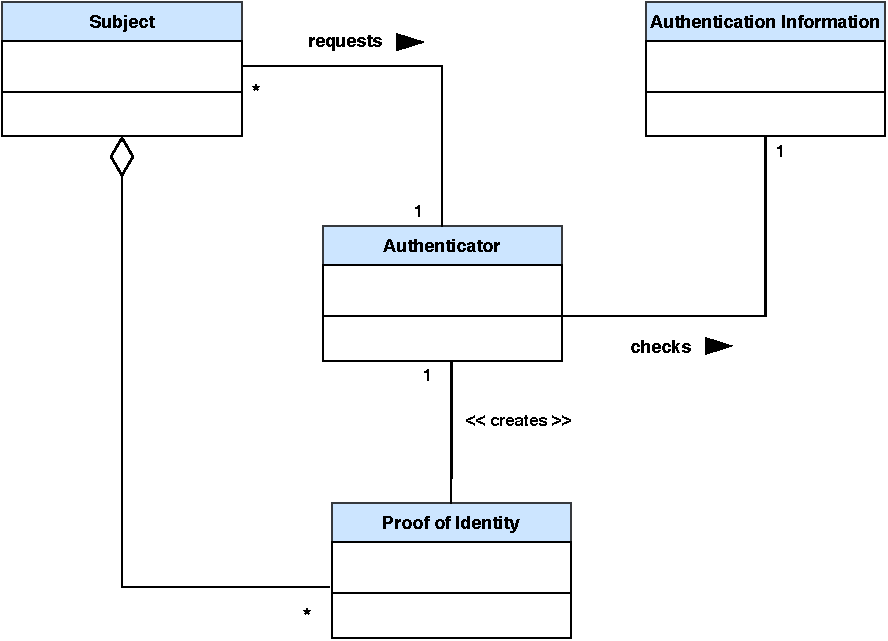
\includegraphics[width=1\columnwidth]{utils/authenticator_CD.pdf}
    \caption{UML class diagram of the Authentication pattern}
    \label{fig:my_label}
\end{figure}

It is composed of four parts:
\begin{itemize}
    \item a \textit{Subject} needing to be authenticated,
    \item a \textit{Proof of Identity}, token given to the subject once the authentication is complete,
    \item an \textit{Authenticator} is the object which implements an authentication algorithm and creates the \textit{Proof of Identity},
    \item \textit{Authentication Information} are the information provided by the \textit{Subject} to the \textit{Authenticator}.

\end{itemize}

%This pattern provides a solution which implicitly separates the \textit{Authenticator} entity from the \textit{Authentication Information}. This type of architecture although more complex is still preferred because it is harder to compromise such a system: an attacker would have to compromise both the \textit{Authenticator} and the \textit{Authentication Information} database to gain access to their expected \textit{Proof of Identity}.

% Sylvain: Expliquer ici que dans le cadre d'une mise en oeuvre de ce pattern, les différents "acteurs" du pattern sont soit des composants déjà existants, soit des composants à aller chercher, soit des composants auxquels fournir des points d'extension, soit des composants à développer, etc... Sinon évidemment on utiliserait des bibliothèques de trucs déjà tout prêts.
%Est-ce que ces détails sont nécessaires pour la suite?

%\subsubsection{Authorization pattern}

%The goal of the Authorization pattern is to identify a subject requesting a resource and to be able to check whether the subject is authorized or not to access it. Once again, the exact nature of the subject and the resource are not defined in the pattern and can be pretty much anything (client and database, user and file access privilege, etc.).

%\begin{figure}
%    \centering
%    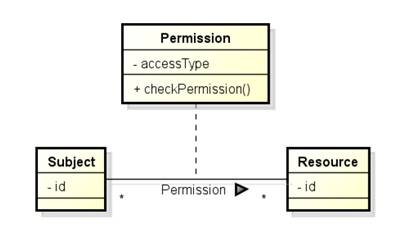
\includegraphics{utils/authorization_CD.png}
%    \caption{UML class diagram of the Authorization pattern}
%    \label{fig:my_label}
%\end{figure}

%This architecture is composed of three entities:
%\begin{itemize}
%    \item the \textit{Subject}, which requires access to a \textit{Resource},
%    \item the \textit{Resource} represents what the \textit{Subject} is allowed to access,
%    \item the \textit{Permission}, which represents one way to access the \textit{Resource} and encapsulates a mechanism to check the validity of the access.
%\end{itemize}

%For this pattern to be relevant, both \textit{Subjects} and \textit{Resources} must be identified in a relevant way: two subjects with the same identifier cannot have different privileges. One way to ensure this property is to give different identifiers to every \textit{Subject} and every \textit{Resource}.
%what does "to be relevant" mean? what does "identified in a relevant way" mean?

%\subsubsection{Pattern composition}
%create a link between the two patterns
%A single and isolated security pattern is usually not enough to secure a system. Thus, multiple security patterns are usually used together, in a process called pattern composition, to improve the security of a software system. For instance, scenarios such as the one in which an application needs to know the identity of the current user and after authentication, it needs to authorize access (to certain resources) to some authenticated users, illustrate a composition process of the Authentication and Authorization security patterns.
% Sylvain: Parler ici de la composition de ces patterns. Mettre en évidence qu'un même composant logiciel peut jour un rôle dans un pattern, et un autre rôle dans un autre pattern

\subsubsection{Limitations of design patterns}\label{PatternLimitations}

The use of design patterns has many advantages for software development as they bring a certain uniformity in software design. They provide a common language between software designers and developers and make software more easily maintainable and extensible. As a generic solution, the definition of a design pattern is usually abstracted from the implementation. Although this abstraction allows for pattern reusability, it is problematic when it comes to security. Indeed, most attacks on software systems are based on weaknesses in the implementation, referred to as vulnerabilities. The presence of natural language in the definition of patterns also introduces potential vulnerabilities, as it is subject to interpretation. In particular, the implementation details are usually implied in the security pattern definition. Therefore, the use of security design patterns does not guarantee the security of a software, as their definition is not formal enough, and thus ambiguous.

\subsection{Design by contract}

The Design by Contract (DbC) concept was coined by Meyer \cite{meyer1992applying} as an approach to design reliable software based on the idea that elements of a software system collaborate with each other on the basis of mutual obligations and benefits.

The whole DbC approach relies on the idea of contract. Meyer indeed realized that most of the software systems, and in particular object-oriented systems, depend on the division of work. This means that tasks are classically divided in several sub-tasks, each being conducted by a program unit. 
%This kind of organization can also be observed in most professional situations. 
Most of the time, the completion of a given task is made possible by the division of labor between several actors. When this happens, the actual interaction of the actors is entirely defined in a \emph{contract}. This contract contains the liabilities and benefits of the interaction for all parties involved. This analogy led Meyer to the idea of software contracting \cite{meyer1992applying}: to define contracts between clients (i.e., routine’s callers) and suppliers (i.e., routines, functions or methods).
A contract is defined as the aggregation of two assertions to a routine or method:
\begin{itemize}
    \item A precondition:  Boolean condition that needs to be verified before calling the routine. It summarizes the client's obligations towards the supplier.
    \item A postcondition: Boolean condition that needs to be verified after the call is made. It summarizes the supplier's obligations towards the client.
\end{itemize}

The whole idea of the DbC approach is that since a contract is formally defined for each service (routine or method), bugs are unlikely to appear at run-time because of a misunderstanding between program units.

In addition to these two assertions, Meyer defined a third type of Boolean expression called a \textit{class invariant}. This notion relies on the class concept. In object-oriented designs, a class should be the representation of some specific concept, usually referred to as object or model. Most of the time, a few properties characterize the essence of the class and should be true at all time and for every instance. A classic example of this idea is the binary tree node class in which all nodes are connected to at most two nodes. A node instance of such a structure should verify at any time that both its children reference it as their respective parent node. This property is then an \textit{Invariant} for this class.

\section{Using cyber contracts to specify security patterns}

The design-by-contract approach \cite{meyer1992applying} states that faults in a software system are the consequence of inadequate programming practices, in contrast to other schools of thought that impute the security problem to even earlier stages of system definition such as requirements elicitation \cite{souag2018Amanda} \cite{mazo2020RSTemplate} \cite{mazo2016framework}and modelling \cite{sun2020domain}. However, this approach was not designed to deal with security issues. Thus, the notion of cyber contract presented in this section, is an extension of the DbC method with concepts coming from the cyber security domain.
In particular, this section (i) formally describes cyber security contracts, (ii) presents the application of such contracts to security patterns, and (iii) develops the case of the authenticator pattern to illustrate our approach.

\subsection{Cyber security contracts}
The core construct of a cyber security contract is the concept of \textit{contract}, which links formal properties and contracting parties as depicted in the  metamodel presented in Figure \ref{fig:CybercontractMetamodel}. The class \textit{Contract} has an attribute \textit{intent}, has a collection of contracting parties and is composed of \textit{Clauses}. The \textit{intent} is a text that describes, in natural language, the purpose of the contract. The contracting parties are represented by the \textit{ContractingParty} class and they correspond to the programming entities whose behaviors are subject to the \textit{Contract}. These entities can be classes, methods, instances, modules, etc. A \textit{Contract}  (i.e., a cyber contract) in our approach differs from the classic view of contracts proposed by Meyer in his DbC paradigm: DbC contracting parties can only be classes and methods whereas ours are not limited by their nature (instances, set of classes, programming units, etc.).. Furthermore, the *-* cardinality in the relation between the \textit{Contract} and \textit{ContractingParty} concepts enables the definition of a \textit{Contract} involving multiple \textit{ContractingParties}, potentially of different nature. This relation also provides the possibility to define multiple contracts for a given \textit{ContractingParty}. In our cyber contract context, the \textit{ContractingParties} stand for the entities involved in the security pattern definition. 

\begin{figure}
    \centering
    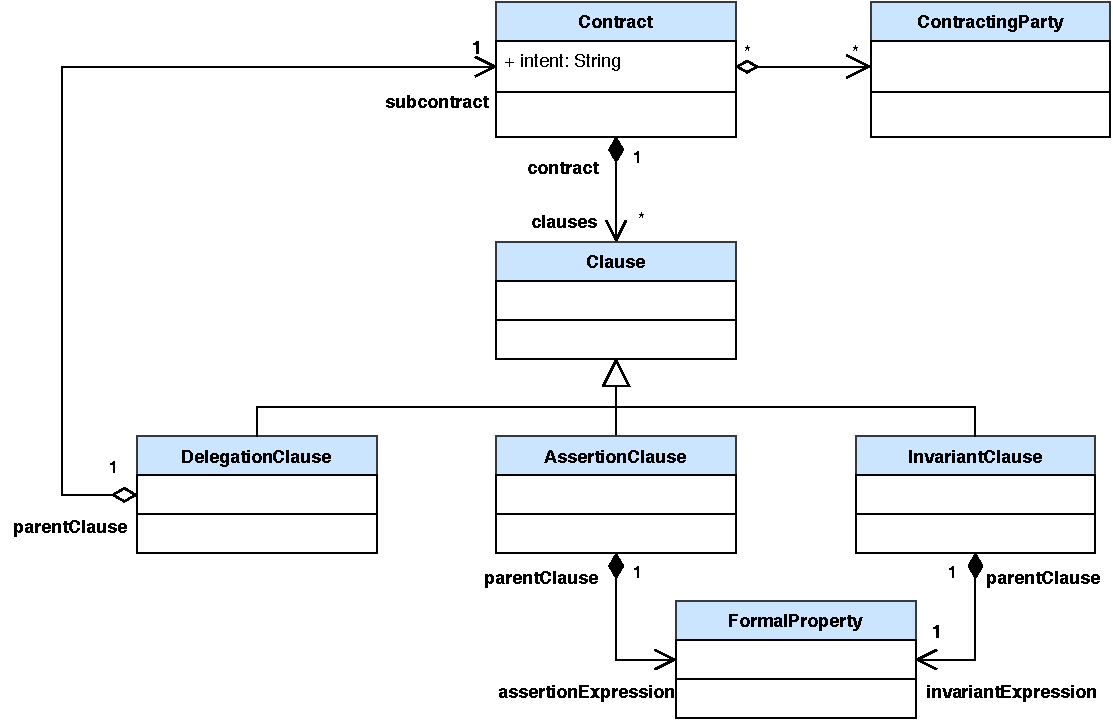
\includegraphics[width=1\columnwidth]{utils/Contract_MM.pdf}
    \caption{Cyber contract metamodel}
    \label{fig:CybercontractMetamodel}
\end{figure}

Every \textit{Contract} is defined as a set of clauses that structure the \textit{FormalProperties} of the corresponding contract \textit{Clauses}. There are three types of \textit{Clauses} that can be added to a \textit{Contract}: \textit{AssertionClause}, \textit{InvariantClause} and \textit{DelegateClause}. 
A \textit{FormalProperty} ensured by the contract refers to one of the two first type of clauses as showed the figure \ref{fig:cybercontractXML} on the Authenticator example.
%The first two clauses wrap a \textit{FormalProperty} which is to be ensured by the contract. 
The \textit{AssertionClauses} enable the specification of assertions that need to be verified at a certain time. They extend the notions of precondition and postcondition of the DbC approach  in a sens that they can be expressed using temporal logic formulas. The \textit{InvariantClauses} are assertions that must always be true, and can therefore be expressed with classical logic. The \textit{DelegateClause} is a concept allowing for responsibilities of a contract to be divided into one or several subcontracts. This mechanism is typically used in the object-oriented paradigm to decompose a contract on the pattern classes, or any decomposition unit of the targeted language.

The last class of the CyberContract metamodel represents the concept of \textit{FormalProperty}. It is an abstraction representing any kind of logic property that one could want to enforce using a contract. In a goal to remain independent of the property expression language, the metamodel does not require any precise expression language.


%Another benefit of our proposal is that a contract can be defined for an assembly of classes, and consequently a security design pattern. Such contract should include all the properties ensuring the correct execution of the pattern. These properties can be functional (i.e., the pattern elements are used in accordance with the pattern description) or implicit  (i.e., a formalization of all implicit meanings of the pattern definition words).

\subsection{Security pattern cybercontract}

Our approach allows for the definition of design pattern contracts. A design pattern is a set of classes and the description of their interactions. We argue that this description can be formalized using a design pattern contract. Such a formalization is particularly relevant regarding security design patterns as presented in Section \ref{PatternLimitations}. 

We have identified two types of formal properties that are relevant to a pattern contract definition: functional and implicit properties.

Functional properties are all the properties expressing the expected behavior of a given pattern. They are the formalization of the interaction of classes as described in the pattern definition. When a pattern is described in natural language, some of the words that are used come with an implicit meaning that can be crucial to the pattern. All these implicit elements, that we call implicit properties, need to be formally expressed in the pattern contract for it to be relevant. A basic example of implicit property is the notion of identifier. Most security design pattern describe fields as identifiers for certain classes. Such identifiers are obviously expected to identify instances of the class. We can for instance define a formal property stating that different instances must have different identifiers. This is an implicit but crucial property.

Thus, as presented in the metamodel, a cyber contract is defined as a set of functional and implicit security properties. The expression of these properties are based on the elements defined in the pattern including classes, instances, attributes and methods. 


\subsection{The Authenticator pattern contract}
\label{label:authenticatorContract}

Let's exemplify the definition of a cybercontract for the Authenticator pattern. To do so, we will use \textit{FormalProperty} expressions based on the object-oriented paradigm for the contract properties.

The \textit{Authenticator} pattern describes a generic authentication mechanism. Six properties have been identified to ensure the security of such a pattern. The first four are implicit properties and the last two are functional properties.
\begin{enumerate}
    \item The first property to check is the uniqueness of the (authentication information, subject) pairs. This property is implicit in the pattern definition but is fundamental. Indeed, if it is not verified, the pattern has no more meaning since an \textit{authentication information} would not identify a unique subject. With $I_{Subject}$ containing all instances of the $Subject$ class, the property can be expressed as follows.
    \begin{equation*}
        P1: \forall a, b \in I_{Subject}, a \ne b \implies a.authInfo \ne b.authInfo
    \end{equation*}
    \item Similarly, since the authentication information is linked to the subject instance, it must not vary during execution (probable identity theft). Let $a.authInfo_{ini}$ be the initial value of the field $authInfo$ of the $Subject$ instance $a$. Formally:
    \begin{equation*}
        P2: \forall a \in I_{Subject}, a.authInfo = a.authInfo_{ini}
    \end{equation*}
    \item A major flaw that can jeopardize authentication systems concerns the non-integrity of the authentication authority. In order to be authenticated, a subject must make a request to the Authenticator. If an attacker succeeds in forging its Authenticator, he becomes master of the authentication system. It is therefore essential that the Authenticator cannot be modified. Thus, let  $a.authenticator_{ini}$ be the initial value of the field $authenticator$ of the $Subject$ instance $a$. This property can then be expressed as follows.
    \begin{equation*}
        P3: \forall a \in I_{Subject}, a.authenticator = a.authenticator_{ini}
    \end{equation*}
    \item At all time, the proof of identity of every subject must be either valid or undefined.
    \begin{equation*}
    \begin{split}
        &P4: \forall a \in I_{Subject}, (a.idProof = \emptyset) \lor \\&(a.idProof = a.authenticator.request(a.authInfo))
    \end{split}
    \end{equation*}
    \item After authentication, the proof of identity must be the one returned by the request method with the correct parameters. According to the DbC approach, it means that the following property should be ensured by the \textit{authenticate} method of the \textit{Subject} class.
    \begin{equation*}
        P5: self.idProof = self.authenticator.request(self.authInfo)
    \end{equation*}
%    \item 
    \item The proof of identity returned by the \textit{request} method of the \textit{Authenticator} class must be valid if and only if the subject requesting it is who it claims to be. More formally, it means that the \textit{request} method must ensure the following property. Let $\emptyset$ be the default value for a variable. The postcondition can then be expressed as follows.
    \begin{equation*}
        P6: self.check(authInfo) \lor returnValue = \emptyset
    \end{equation*}
\end{enumerate}

Figure \ref{fig:cybercontractXML} shows a simplified XML representation of this contract.
This representation illustrates an instantiation of our metamodel on the Authenticator cyber contract. The binding with the Authenticator pattern is explicit and we can see the property P1 as an \textit{InvariantClause} defined at the pattern scope.
The delegation mechanism provided with the \textit{DelegateClauses} is also illustrated within this example. Some of the previous properties are indeed within the scope of a single method (P5 and P6). They are thus delegated to the relevant classes using a \textit{DelegateClause} (keyword \textit{Subcontract}) and then to the correct methods.

%For example purposes, let's consider one possible expression language for the \textit{FormalProperty} concept, base on the object-oriented paradigm. This expression language will then be used to define the cybercontract of the Authenticator pattern, described with the object-oriented paradigm.
%si j'ai bien compris, ce qu'on a voulu faire ici c'est de présenter un exemple de l'utilisation de ce concept dans le cas du Authentication patten. Si c'est cela voici comme on dévrait présenter la chose:
%Let's show the implementation of a proof of concept for the \textit{FormalProperty} class. To do so, let's consider the Authenticator pattern, implemented in an object-oriented language, to represent the formal properties corresponding to its CyberContract.
%et ensuite on présente tout ce qu'il y a dans la section Authenticator CyberContract (sans être une section mais comme une continuation de cette sub-section) et la partie $I_{Class}$, $var_{ini}$ et $\emptyset$ on la présente au moment de l'utilisation de chaque concept avec un Where $\emptyset$ represents  the... car avec la manière comme on est en train de présenter la chose on les oublie tout de suite et ça fait revenir le lecteur pour consulter la def de chaque chose et cela est très genant.
%Let's consider the following notations for the properties:
%\begin{itemize}
%    \item Let $I_{Class}$ be the set containing all instances of the class $Class$.
%    \item Let $var_{ini}$ be the initial value (right after the constructor call) of the variable $var$.
%    \item Let $\emptyset$ be the undefined state for a variable.
%\end{itemize}
%As for the logic system of the properties, the contract \textit{Boolean expressions} use the mathematical operators $\forall$ and $\exists$ along with classical Boolean operators ($\implies$, $\land$, etc.).

%Let's now consider the  Authenticator pattern 

%ici il faut préparer le lecteur à la section suivante car le changement est très abrupt (je vais lire la section pour savoir ce qu'elle présente et voir si je peux faire ici le lien)

\begin{figure}
    \centering
 \begin{lstlisting}[breaklines=true, language=XML, basicstyle=\ttfamily\footnotesize, mathescape=true]
<Contract>
    <binding "Authenticator_pattern" />  
    <clauses> 
    <InvariantClause P1/>  
    <Subcontract "SubjectContract">
        <binding "Subject" />
        <InvariantClause P2 $\land$ P3 $\land$ P4/>
        <Subcontract "authenticateContract"s>
            <binding "void authenticate()">
            <ensures P5/>
        </Subcontract>
    </Subcontract>
    <Subcontract "AuthenticatorContract">
        <binding "Authenticator"/>
        <Subcontract "requestContract">
            <binding = "ProofOfIdentity request(AuthenticationInformation authInfo)">
            <ensures P6/>
        </Subcontract>
    </Subcontract>
    </clauses>
</Contract>

\end{lstlisting}
\begin{equation}
\begin{split}
\\
&P1: \forall a, b \in I_{Subject},a \ne b \implies a.authInfo \ne b.authInfo\\
&P2: \forall a \in I_{Subject}, a.authInfo = a.authInfo_{ini}\\
&P3: \forall a \in I_{Subject}, a.authenticator = a. authenticator_{ini}\\
&P4: \forall a \in I_{Subject}, a.idProof = \emptyset \lor \\
&a.idProof = authenticator.request(authInfo)\\
&P5: self.idProof = self.authenticator.request(self.authInfo)\\
&P6: self.check(authInfo) \lor returnValue = \emptyset
\end{split}
\nonumber
\end{equation}
\caption{XML representation of the Authenticator pattern contract}
\label{fig:cybercontractXML}
\end{figure}


\section{PAMELA approach for specification and run-time monitoring of cyber-contracts}
%\section{Experiments and preliminary evaluation}

In this section, we show how our approach can be mapped on two frameworks to specify cyber-contracts on security patterns and we show how to use them on existing code.
%This section discusses the implementation of our approach in two different languages as well as a preliminary evaluation study.

In particular, our approach was implemented in two software specification languages. Both implementations enable the addition of an extra layer of trust in the existing code, to enforce the formal properties of predefined security design patterns, without the need to modify the code. We implemented our approach in the Java Modelling Language (JML) \cite{leavens2006}, a DbC-based specification language, and PAMELA, a Java modelling language and framework \cite{PAMELAWebSite}.

These two languages were selected on the basis of an existing active community, the relevance regarding our approach and their ability to be extended without having to enrich or modify the syntax of the hosting language.

\subsection{Java modelling language experiment}
%Our design by contract approach to specify security patterns was implemented in two software specification languages. In particular, both implementations enable the addition of an extra layer of trust in the code of a system to enforce the formal properties of existing security design patterns without the need to modify the code. We implemented our approach in the Java Modelling Language (JML), a DbC-based specification language, and PAMELA, a framework to ...
%These two languages were selected on the basis of their popularity and their ability to be extended without having to enrich or modify the syntax of the language.
%We started from the observation that in most cases, existing code implements forms of security patterns without naming them. The objective was therefore to develop to show that it was possible to start from an existing code and secure it without much modification. The securing in question is of course linked to the notion of contracts. I therefore followed two successive approaches to secure existing code. The first approach consists in implementing the contracts with JML (Java Modelling Language). The second is the implementation of security patterns in the PAMELA framework.

%\subsubsection{Java modelling language implementation}
Java Modelling Language (JML) \cite{leavens2006,cok2014} is a specification language  that enables engineers to write DbC assertions as comments in Java code. These comments are then parsed by a specific compiler (called JMLC). The resulting java bytecode is the aggregation of java compile code and java assertions enforcing JML expressions.
The JML language allows referencing the namespace of the Java program and the logical operators of the Java language. It also has some keywords and symbols that correspond, for the most part, to the concepts of the DbC approach. For example:
\begin{itemize}
    \item \textit{forall}, \textit{exist}, $=>$ and $<=>$, which correspond to the universal quantification, existential quantification, and logical implication and equivalence, respectively;
    \item \textit{invariant}, \textit{requires} and \textit{ensures} are used to represent, respectively, the invariants, preconditions and postconditions of contracts;
    \item assignable \textit{<name>} to specify that a variable can be assigned in the method it specifies;;
    \item \textit{old<name>} to reference the value of a variable before the call of the method it specifies;
    \item \textit{result} to reference the return value of the method it specifies;
    \item \textit{signals} describes the exceptions thrown by the method it specifies;
    \item \textit{pure} specifies that the specified method does not have side effects;
    \item \textit{also}: declares that a method inherits JML specification (preconditions and postconditions) from its supertype and adds specific specifications.
\end{itemize}

We use OpenJML \cite{cok2014} as the tool support to create the logical annotations in existing Java programs. In addition, it enables static or run-time checking of the validity of the annotations through static code verification and dynamic assertion checking capabilities.
%Pas sur de comprendre ce que tu veux dire par là. JML est le langage, JMLC le compilateur et openJML le framework qui permet de faire de la vérification formelle sur du code JML.


The rest of this subsection shows how to specify the \textit{Authenticator} pattern as a cyber-security contract with JML and some lessons learned from this experience. 

To specify the \textit{Authenticator} pattern as a cyber-security contract with JML, the six formal properties presented in Section \ref{label:authenticatorContract} are implemented through JML expressions, as presented below:
\begin{enumerate}
    \item Uniqueness of authentication information
    \begin{equation*}
        P1: \forall a, b \in I_{Subject},a \ne b \implies a.authInfo  \ne b.authInfo 
    \end{equation*}
    This property illustrates one of the limitations of the standard DbC approach and consequently the JML framework, in which a property is limited to be expressed for the scope of a class or a method, and so relative to one instance. As a result, this property cannot be expressed in JML since a JML expression is limited to the scope of a class and cannot involve more than one instance of the corresponding class.
    %To overcome this constraint, the code of the pattern must be expanded on adding code which impact the pattern classes.
    
    \item Invariance of authentication information
    \begin{equation*}
        P2: \forall a \in I_{Subject}, a.authInfo = a.authInfo_{ini}
    \end{equation*}
    This property is conceptually an invariant of the \textit{Subject} class. It however requires to know, at all time, what is the initial value of the \textit{authenticationInformation} field. One way to implement this "memory" in JML is to add the following ensure clause to every method, except the constructor, of the \textit{Subject} class. The constructor call does not support the use of $\backslash$old(authInfo) keyword. This is why we cannot use an invariant clause.
    \begin{center}
        \textit{@ ensures authInfo == $\backslash$old(authInfo);}
    \end{center}
    
    \item Invariance of authenticator
    \begin{equation*}
        P3: \forall a \in I_{Subject}, a.authenticator = a.authenticator_{ini}
    \end{equation*}
    This property can be implemented similarly to the previous one with the following ensure clause for every method of the \textit{Subject} class.
    \begin{center}
        \textit{@ ensures authenticator == $\backslash$old(authenticator);}
    \end{center}
    
    \item Validity of the Proof of Identity
    \begin{equation*}
    \begin{split}
        &P4: \forall a \in I_{Subject}, (a.idProof = \emptyset) \lor \\&(a.idProof = a.authenticator.request(a.authInfo))
    \end{split}
    \end{equation*}
    This property can be transposed to the following JML invariant for the \textit{Subject} class.
    \begin{center}
        \textit{@ invariant idProof == null || idProof == authenticator.request(authInfo);}
    \end{center}
    
    \item Correctness of authenticate method
    \begin{equation*}
        P5: self.idProof = self.authenticator.request(self.authInfo)
    \end{equation*}
    This property is directly a JML postcondition for the \textit{authenticate} method of the \textit{Subject} class.
    \begin{center}
        \textit{@ ensures idProof == authenticator.request(authInfo);}
    \end{center}
    
    \item Correctness of the request method
    \begin{equation*}
        P6: self.check(authInfo) \lor returnValue = \emptyset
    \end{equation*}
    This property is also a JML postcondition for the \textit{request} method of the \textit{Authenticator} class.
     \begin{center}
        \textit{@ ensures check(authInfo)} || \textit{$\backslash$result == null;}
    \end{center}
\end{enumerate}

%JML Implementation results and lessons learned
Regarding our approach, the previous example highlights the limitations of the standard DbC approach and consequently the JML framework. More specifically, there are two main expression issues that cannot be solved. The first is the limitation of a JML contract to the scope of a class or a method . This restriction prevents the expression of any contract property involving more than one instance of a class. The second issue has to do with the lack of memory of the JML-based DbC approach. Indeed, in JML, a DbC property can only refer to the current state of an instance, or in the case of the post or precondition of a method, to the state before the call of the method. The previous examples show that we sometimes need to have an evolving state for the scope of the contract properties. This could be managed for instance by implementing pattern objects that could enforce the contract properties. 
% ?? (retiré sans être sur mais ici on donne la solution de Pamela) In particular, these objects would have an evolving state and could therefore save any information relevant to their associated contract properties and at any moment of the execution.
%Caine: Generalize as to what the limitations of JML-based properties are. 

\subsection{The PAMELA experiment}

%\subsubsection{The PAMELA framework}

PAMELA is a Java modelling framework developed by the Openflexo community \footnote{https://www.openflexo.org}. This project aims at bridging the gap between software modelling and code implementation. 
%In the context of Model-Driven Engineering (MDE), the generative approach is promoted from a domain model to a dedicated model or a custom application source code. 
% TODO: @Joel: que veux-tu dire là ???
%This gap includes generally a semantic gap, because semantics may be hidden or remains implicit in the transformation. %Another drawback is the development or maintenance process, where model and source code must evolve independently and complex round-tripping mechanisms must be enforced. 

In this context, PAMELA modelling framework proposes an approach where models are directly weaved in source code, by means of Java annotations. Thus, it does not require code generation. That way, both model and source-code coexist in the same artifact. 
%A major challenge to be addressed by MDE approaches is the ability to integrate custom implementation to a base of code derived from a domain model. 
%PAMELA framework allows the use of common extension points such as inheritance, as offered by the Java language, and provides a way to define some partial implementations (a set of methods), easing coupling between formal behaviour as specified in the domain model, and custom implementations.
%PAMELA framework provides a way to define a domain model and its associated code separately from the application code. 
%The annotation support allows an easy and flexible coupling of the specified domain model and custom implementation.

\begin{figure}
    \centering
    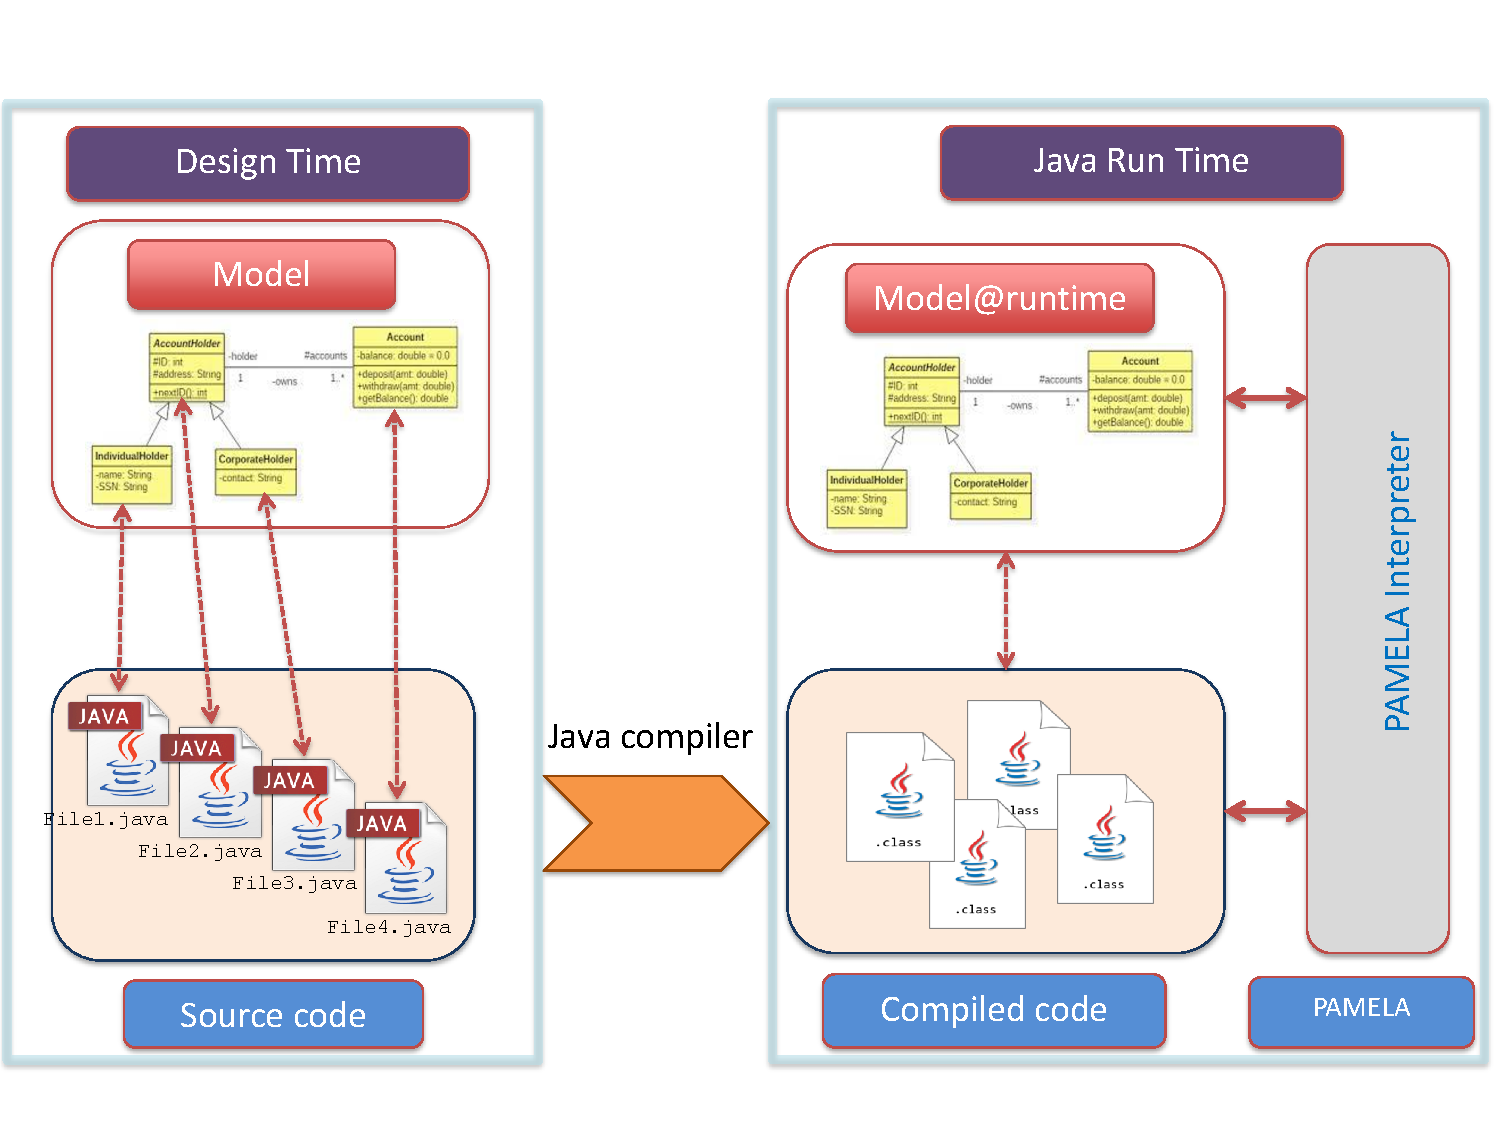
\includegraphics[width=1.0 \columnwidth]{utils/PamelaVisionV2.pdf}
    \caption{Overview of the PAMELA approach}
    \label{fig:PamelaVision}
\end{figure}

Figure \ref{fig:PamelaVision} illustrates the PAMELA framework where we have at design time (left side of the figure), the model weaved in source code files based on the Java annotations and at run-time (right side of the figure) the PAMELA interpreter ensuring the link between the model behavior and the application Java byte-code.

Resulting execution is a combination of (i) executing plain Java byte-code as the result of the basic compilation of source code, and (ii) an embedded PAMELA interpreter executing PAMELA model semantics.
 
From an implementation standpoint, PAMELA uses \emph{javassist} reflection library including the \texttt{MethodHandler} mechanism. Based on this support, the Java dynamic binding is overridden to provide the call of the PAMELA model behavior when an object method is invoked. 
%which is part of a PAMELA model caused the real implementation to be called when existing (more precisely dispatch code execution between all provided implementations), or the required interpretation according to underlying model to be executed. This provides also an extension point allowing to instrument the code, which is used for other features such as undo/redo stack management, and allows assertion checking at run-time. PAMELA framework is a 100\% pure Java (> 1.5), compilable by a classical Java compiler and executable in a classical Java virtual machine.


%\subsubsection{PAMELA \emph{Patterns}}

PAMELA framework offers some Aspect-Oriented Programming (AOP) features enabling the definition of additional behaviour to existing Java code. 

%We define a \emph{Pattern} as a composite of multiple stakeholders, whose roles are played by various Java classes. A \emph{Pattern} regroup and implement all concerns related to concept association, which are orthogonal to each functional class concern. Each method of involved classes can be considered as a \emph{pointcut} as of AOP terminology. Such \emph{Pattern} is instantiated, and provides a statefull environment. Code instrumentation and code weaving are operated at run-time by PAMELA interpreter. A \emph{Pattern} comes with its business logic (acting on control flow of all pattern-related methods), and a set of assertions (invariants, pre-conditions and post-conditions) which are evaluated at run-time, while functional code is executed.

%We choose to implement our approach with PAMELA \emph{Patterns} because this scheme perfectly fits our requirements:
%\begin{itemize}
%    \item the ability to use existing plain Java code, without any restriction,
%    \item existing code can be instrumented (PAMELA provide handlers both at entry and exit of methods execution, allowing execution of pre and post conditions),
%    \item pattern can offer some structural and behavioural features, executed by PAMELA interpreter, 
%    \item patterns are instantiated and provides statefull environment, allowing the computation of assertions using many paradigms (e.g., Linear Temporal Logic),
%    \item PAMELA offers multiple extension points: ability to redefine or specialize an existing pattern, and ability to provide a new pattern definition.
%\end{itemize}

We chose to extend the PAMELA framework to include our notion of \emph{Pattern}, i.e. a composition of multiple classes, known as \emph{Stakeholders}, whose expected behavior is defined in a pattern contract, along with formal properties which must be ensured at run-time. More specifically, implementing \emph{Patterns} with PAMELA provides:
\begin{itemize}
    \item the ability to use existing plain Java code, without any restriction;
    \item the ability to monitor the execution of the code;
    \item the ability to offer extra structural and behavioral features, executed by the PAMELA interpreter;
    \item a representation of \emph{Patterns} as stateful objects. Such objects can then evolve throughout run-time and compute assertions using any paradigms (e.g., LTL - Linear Temporal Logic);
    \item the ability of having multiple extension points. In other words, the ability to create new patterns, or to redefine or specialize existing ones.
\end{itemize}

\emph{Patterns} are defined in PAMELA using three classes, each one representing a different conceptual level:
\begin{itemize}
    \item a \mytexttt{PatternFactory}. This class is responsible for identifying, at run-time, the declared patterns in the Java byte-code.
    \item a \mytexttt{PatternDefinition}. This class represents an occurrence of the pattern in the supplied byte-code. It has the responsibility of maintaining links with all classes and methods involved in the pattern, as well as managing the life-cycle of its \mytexttt{PatternInstances}.
    \item a \mytexttt{PatternInstance}. This class represents the instance of a pattern at run-time. It is responsible for maintaining the pattern state and providing pattern behavior and contract enforcement.
\end{itemize}

To declare a \emph{Pattern} on existing code, pattern elements such as \emph{Pattern Stakeholders} and methods need to be annotated with provided pattern-specific  annotations. These annotations will be discovered at run-time by the \mytexttt{PatternFactory} and stored in \mytexttt{PatternDefinition} attributes.

\begin{figure}
    \centering
    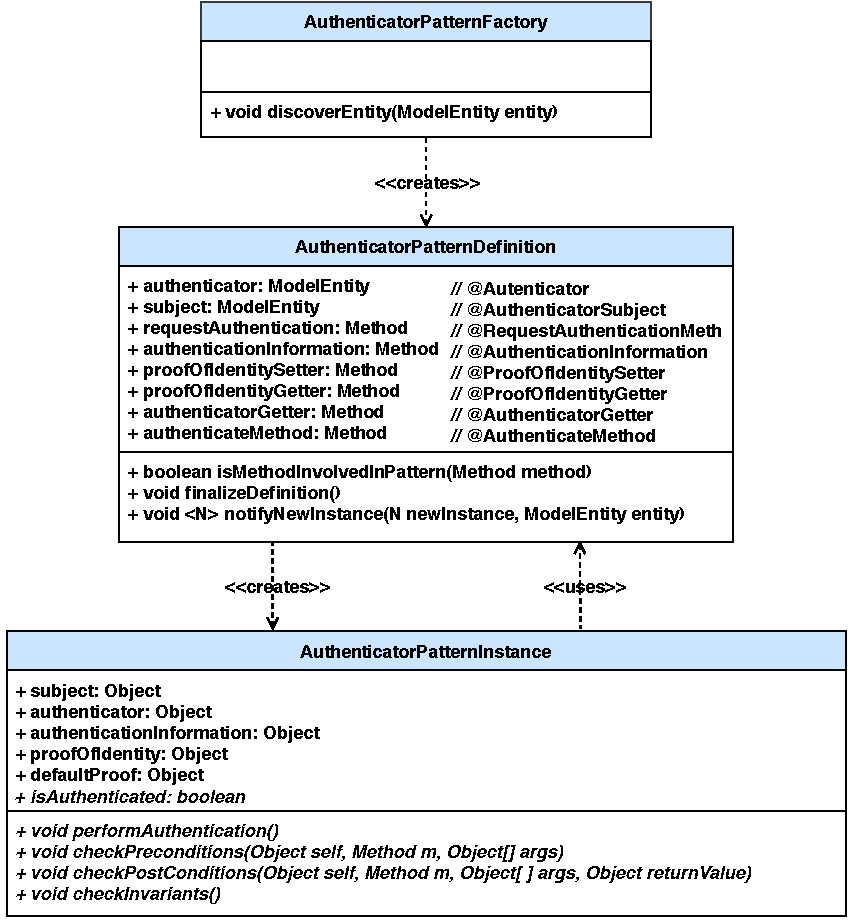
\includegraphics[width=0.8 \columnwidth]{utils/PAMELAAuthenticator_CD.pdf}
    \caption{PAMELA Authenticator pattern class diagram. Emphasized attributes and methods are the one referenced in Figure \ref{fig:AuthenticatorControlFlow}.}
    \label{fig:PAMELAAuthenticator_CD}
\end{figure}

To validate the implementation of our approach in PAMELA we propose an implementation of the \emph{Authenticator pattern} as a cyber-security contract. Figure \ref{fig:PAMELAAuthenticator_CD} presents the previous class structure in the case of the Authenticator pattern. Note that each attribute of the \mytexttt{AuthenticatorPatternDefinition} class has a corresponding annotation (displayed as a comment).

\begin{figure}
    \centering
    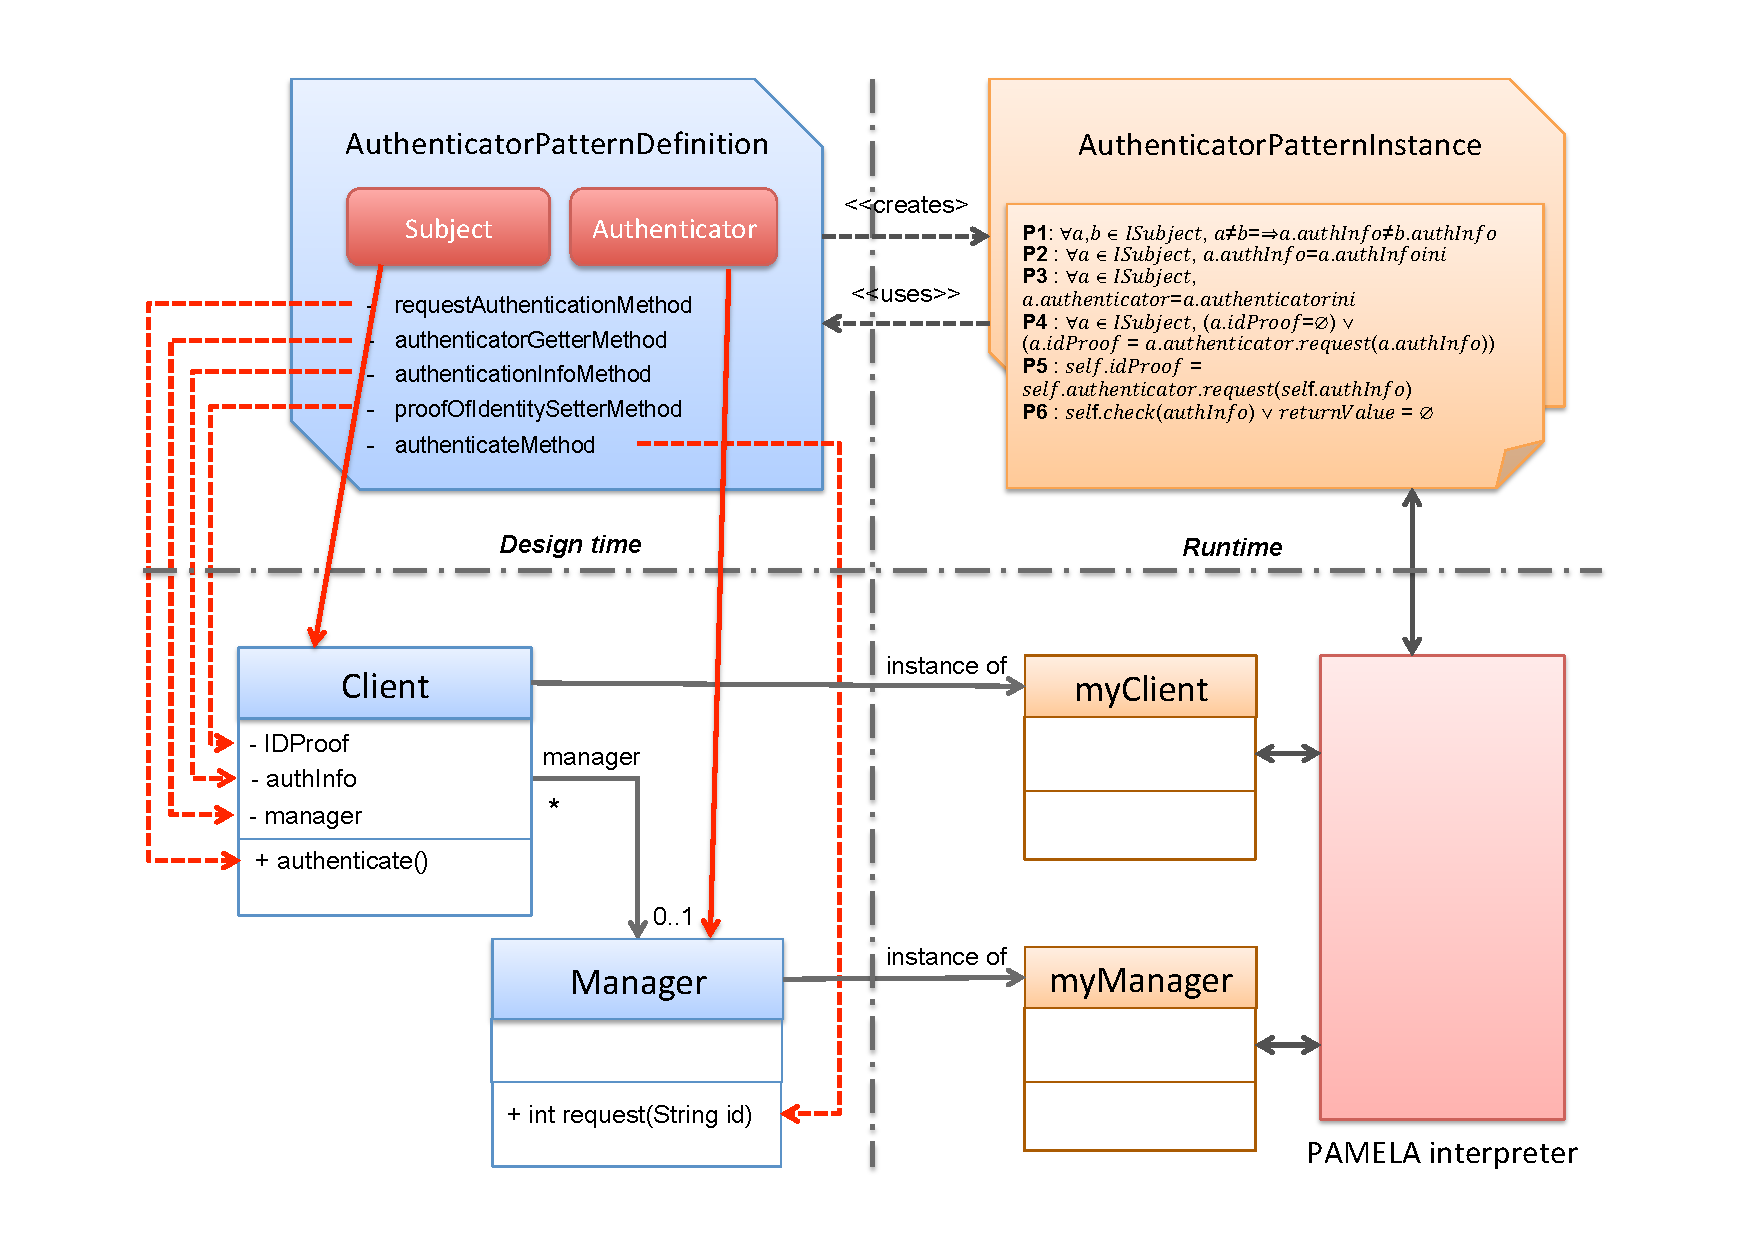
\includegraphics[width=1.0 \columnwidth]{AuthenticatorPattern4.pdf}
    \caption{PAMELA vision of the authenticator pattern}
    \label{fig:AuthenticatorPattern}
\end{figure}

Figure \ref{fig:AuthenticatorPattern} presents the composition of the \emph{Authenticator} pattern with an existing base of code. The  \emph{Authenticator pattern} requires the definition of two \emph{stakeholders} (\emph{Authenticator} role and \emph{Subject} role) which have to be played by instances of provided Java classes. A set of annotations coming with the \emph{security pattern} definition is used to explicit that roles (respectively \texttt{@Authenticator} and \texttt{@AuthenticatorSubject} annotations). The definition of the pattern also requires the distribution of responsibilities and relationships according to the underlying semantics of the pattern (here, the authentication concerns). The request authentication method is identified using the \texttt{@RequestAuthentication} annotation. In the same way, we must identify some responsibilities in the \texttt{Client} class: the method providing the  \emph{Authenticator} access, the method providing the authentication information, the method setting the proof of identity and the \mytexttt{authenticate()} method itself.

%With that implementation, contract assertions do not require to be explicitly defined by the programmer, but are inherent to the security pattern, and are encoded in plain Java code. From an operational point of view, the security pattern is reified as a Java instance, and maintains a statefull environment on which contract assertions may be defined.


The excerpt of code presented Figure \ref{fig:ExampleOfAuthenticatorPattern} shows how the Authenticator pattern is used by means of annotations to an existing base of code. An instance of the \texttt{Manager} class plays the \emph{Authenticator} role, while an instance of the \texttt{Client} class plays the \emph{Subject} role.

\begin{figure}
    \centering
\begin{lstlisting}[language=Java,basicstyle=\ttfamily\footnotesize]
@ModelEntity
@Authenticator(patternID = "MyPatternId")
public class Manager {

	@RequestAuthentication(patternID = "MyPatternId")
	public int request(@AuthenticationInformation(patternID = "MyPatternId", paramID = "id") String id) {
		return ...;
	}
}

@ModelEntity
@AuthenticatorSubject(patternID = "MyPatternId")
public class Client {

	public Client(Manager authenticator, String id) {
		...
	}

	@AuthenticationInformation(patternID = "MyPatternId", paramID = "id")
	public String getAuthInfo() {
		return ...;
	}

	@ProofOfIdentityGetter(patternID = "MyPatternId")
	public int getIDProof() {
		return ...;
	}

	@AuthenticatorGetter(patternID = "MyPatternId")
	public Manager getManager() {
		return ...;
	}

	@AuthenticateMethod(patternID = "MyPatternId")
	public void authenticate() {
		setIDProof(getManager().request(getAuthInfo()));
	}

	@RequiresAuthentication
	public void securedMethod() {
		...
	}
}
\end{lstlisting}
    \caption{Example showing how to use the Authenticator pattern defined as a PAMELA cyber-contract}
    \label{fig:ExampleOfAuthenticatorPattern}
\end{figure}

%\emph{Authenticator} pattern implementation is provided by a Java implementation gathering three classes representing a different conceptual level as defined in the Meta-Object Facility (MOF):
%\begin{itemize}
%    \item \texttt{AuthenticatorPatternFactory.java} (layer M2) : provides features to identify in byte-code at run-time the implementation of an \emph{Authenticator} pattern, on the basis of \texttt{patternId} identifier.
%    \item \texttt{AuthenticatorPatternDefinition.java} (layer M1) : represents an occurrence of \emph{Authenticator} pattern in supplied byte-code. This class has the responsability of maintaining links with classes and methods involved in pattern, as well as managing life-cycle of that pattern instances. 
%   \item \texttt{AuthenticatorPatternInstance.java} (layer M0) : represents an instance of \emph{AuthenticatorPatternDefinition} pattern. This class has the responsability of maintaining state of pattern instance, and managing  business logic as offered by the pattern.
%\end{itemize}

%In the context of \emph{Contract Programming}, this is the AuthenticatorPatternInstance class which has the responsability of defining and checking at run-time the different contract clauses (invariants, preconditions and postconditions). Note that contrary to the JML implementation of our approach, the programmer does not have to define the contract clauses, which are hard-coded in pattern implementation.

%\subsubsection{PAMELA \emph{Patterns} Caine}

%We chose to extend the PAMELA framework to include our notion of \emph{Pattern}, i.e. a composition of multiple classes, knwon as \emph{Stakeholders}, whose expected behavior is defined in a pattern contract, along with formal properties which must be ensured at run-time. More specifically, the implemented PAMELA \emph{Pattern} feature provides:
%\begin{itemize}
%    \item the ability to use existing plain Java code, without any restriction;  \emph{Pattern}
%    \item the ability to monitor the execution of the code;
%    \item the ability to offer extra structural and behavioral features, executed by the PAMELA interpreter, 
%    \item a representation of \emph{Patterns} as stateful objects. Such objects can then evolve throughout run-time and allow the computation of assertions using many paradigms (e.g., Linear Temporal Logic);
%    \item multiple extension points: ability to redefine or specialize an existing pattern, and ability to provide a new pattern definition.
%\end{itemize}

%\emph{Patterns} are defined in PAMELA using three classes, each representing a different conceptual level:
%\begin{itemize}
%    \item a \mytexttt{PatternFactory}. This class provides features to identify in the java byte-code, at run-time, the declared patterns.
%    \item a \mytexttt{PatternDefinition}. This class represents an occurrence of the pattern in the supplied byte-code. It has the responsibility of maintaining links with all classes and methods involved in the pattern, as well as managing the life-cycle of its \mytexttt{PatternInstances}.
%    \item a \mytexttt{PatternInstance}. This class represents the instance of a pattern at run-time. It is responsible for maintaining the pattern state and providing pattern behavior and contract enforcement.
%\end{itemize}

%To declare a \emph{Pattern} on an existing code, pattern elements, i.e. \emph{Pattern Stakeholders} and methods, need to be annotated with provided pattern-specific Java annotations. These annotations will then be discovered at run-time by the \mytexttt{PatternFactory} and stored in \mytexttt{PatternDefinition} attributes. 

%The figure \ref{fig:PAMELAAuthenticator_CD} presents the previous structure in the case of the Authenticator pattern. Note that all attributes of the \mytexttt{AuthenticatorPatternDefinition} class are associated with an annotation (displayed as commentaries).
%\begin{figure}
%    \centering
%    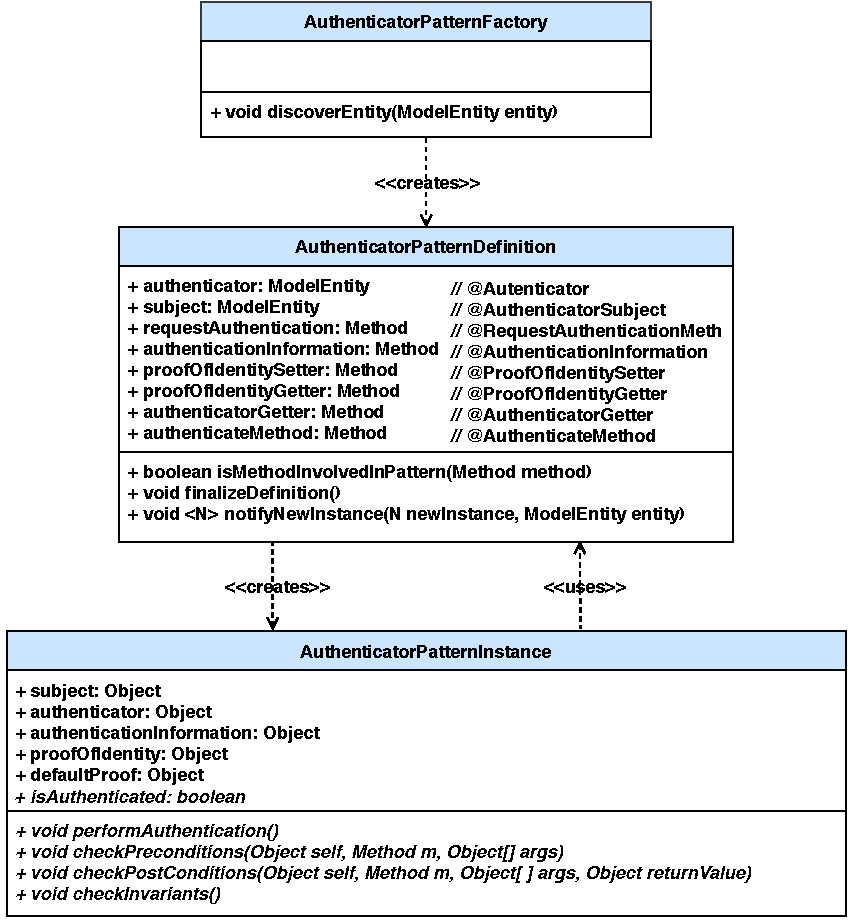
\includegraphics[width=1.0 \columnwidth]{utils/PAMELAAuthenticator_CD.pdf}
%    \caption{PAMELA Authenticator pattern class diagram}
%    \label{fig:PAMELAAuthenticator_CD}
%\end{figure}

At run-time, both functional code and security pattern logic, i.e pattern behavior and contract enforcement, are weaved by the PAMELA framework. 

%More specifically, \mytexttt{PatternDefinition} classes implement the \mytexttt{isMethodInvolvedInPattern} which returns \mytexttt{true} for all methods which need to be handled by the associated \mytexttt{PatternInstances}. This allows, for instance, for the pattern contract properties to be checked at run-time before and/or after any method of interest. In the case of the Authenticator pattern, the \texttt{AuthenticatorPatternInstance} objects will check the invariants of the pattern contract before and after every call to \emph{Subject} and \emph{Authenticator} classes. These checks are performed by the \texttt{checkInvariant} method. 

This implementation, unlike JML, provides a contract enforcement mechanism which is hard-coded within PAMELA \emph{Pattern} classes. This abstraction is closer to the requirements of the end-user, who may want to add an authentication mechanism to an existing code. The user only need to annotate his code and PAMELA will automatically handle the pattern business logic (both, pattern behavior and assertion checking).

\begin{figure}
    \centering
    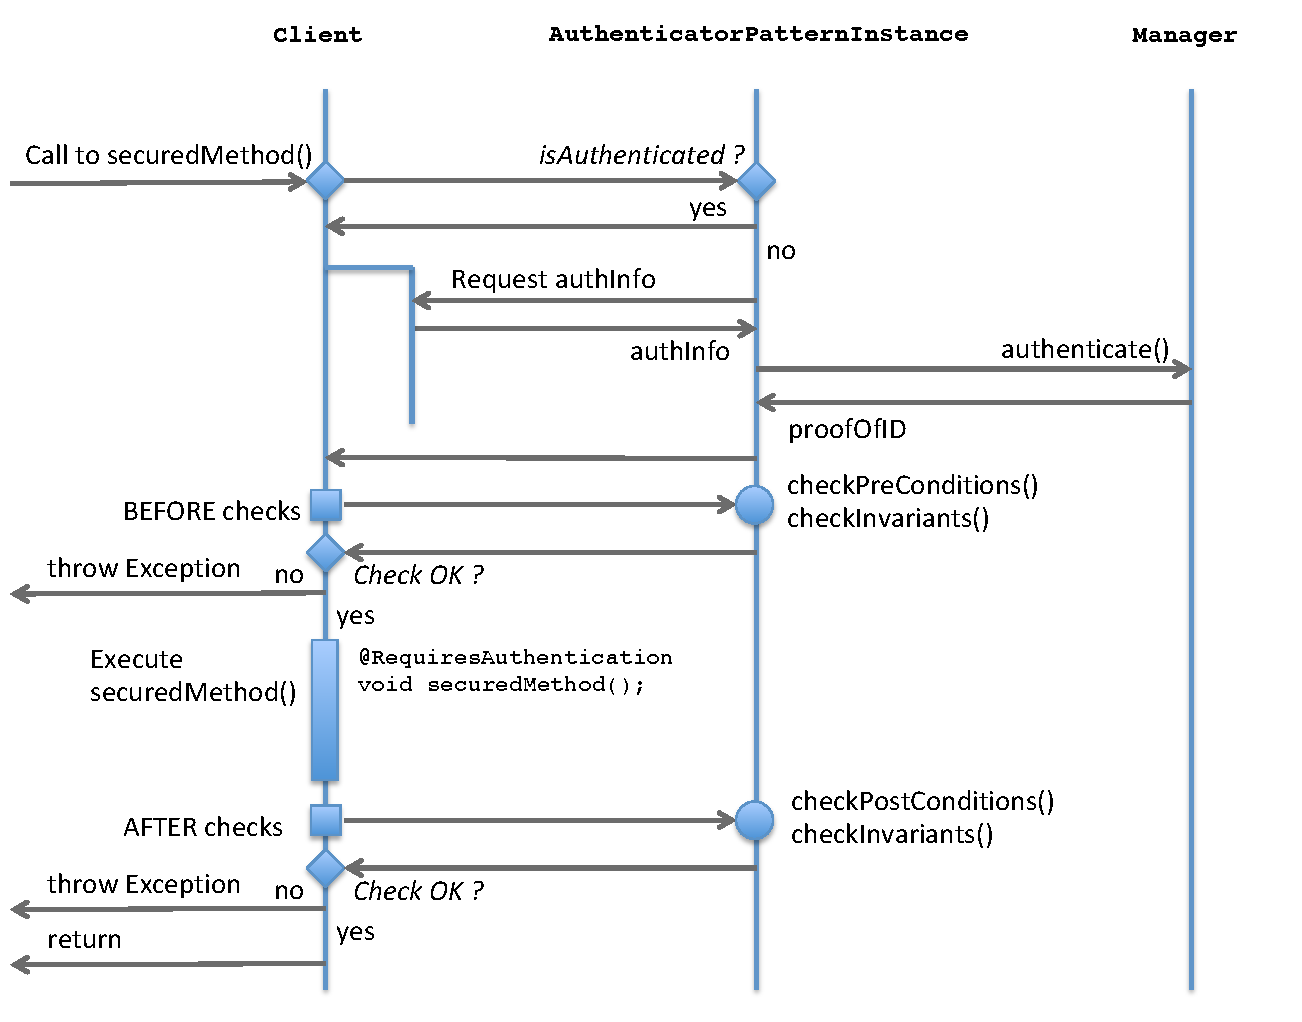
\includegraphics[width=1.0 \columnwidth]{AuthenticatorControlFlow.pdf}
    \caption{Authenticator control flow}
    \label{fig:AuthenticatorControlFlow}
\end{figure}

Figure \ref{fig:AuthenticatorControlFlow} depicts  the control flow of the execution of a method annotated with \mytexttt{@RequiresAuthentication}. 
This annotation is used to identify methods which must trigger the authentication process before being executed. The call will thus be handled as follows:
\begin{itemize}
	\item The method is identified as a method of interest because this method requires authentication.
	\item The method is passed to the relevant \mytexttt{AuthenticatorPatternInstance} (second object on the Figure) before the method execution.
	\item The authentication process is to be executed, because subject is not authenticated yet (\mytexttt{isAuthenticated} is \mytexttt{false}).
	\item Before executing the called method, contract invariants are checked (properties P1 to P4) via the \mytexttt{checkInvariants()} call. If a clause breach is detected, an exception is thrown and the method is not executed. This is also at this time that preconditions are checked (method \mytexttt{checkPreConditions}).
	\item The method is invoked.
	\item The method is once again passed to the \mytexttt{AuthenticatorPatternInstance} after the method execution. Contract invariants are checked. If a clause breach is detected, an exception is thrown. Similarly,  post-conditions are checked (method \mytexttt{checkPostConditions}).
	\item Finally, the result of the method is returned to the caller.
\end{itemize}

%PAMELA implementation results and lessons learned
\subsection{Lessons learned from experiments}

% lessons learned regarding the challenges of the introduction
The two experiments emphasize that the formal behavioral definition of security contracts is an efficient approach to provide several implementations based on our design by contract definition.

The JML experiment highlights the limitations of this DbC implementation for security pattern contract definition. DbC implementations are too limited and fail to express properties requiring multiple class instances or an evolving pattern state. This justifies  the necessity to extend the scope of contract definitions to more complex contracting parties, such as sets of classes. 

These limitations are overcome with the PAMELA approach which provides the ability to freely build models based on multiple  classes with their own semantics and behavioral code.
In this case, our security cyber-contracts are applied at the top of the set of classes used in the security pattern.  
%The PAMELA experiment points out the capacity to allow (i) the verification, at run-time, of clauses involving universal and existential quantifiers on a set of instances and (ii) the support of temporal clauses on stateful instances. 

Regarding the challenges we wanted to target, PAMELA provides an efficient and easy framework to apply security patterns using Java annotations . This can be done at a very early stage of design process of a software component, but this framework can also be applied on legacy source code beeing annotated.

Securing existing code remains a difficult task but our proposal, based on both formal behavioral contract and run-time property enforcement, enforces the security of software components.

%\begin{itemize}
%    \item Structural boundary limitations observed with JML do not apply here, because a pattern may involve an arbitrary instances of different classes playing a role.
%    \item PAMELA offers a run-time access to all instances of patterns and their definitions, allowing verification of clauses involving universal and existential quantifiers. 
%    \item Because pattern instances are statefull, we may consider temporal assertions (such as Linear Temporal Logic formalism).
%\end{itemize}

%Application to \emph{SecurityPatterns} offers the way to provide a secured run-time environment where calls to functional code are dynamically weaved with security pattern internal policy, and are guarded with run-time verification of some security assertions.

%\subsection{Evaluation}

%\subsubsection{Cases}

%To evaluate our approach, we conducted a set
%of experiments on two cases: ...

%\subsubsection{Effectiveness}

%To determine the effectiveness of the approach, we measure the ... of each case. In Figure X and Figure Y, we present the results of ... The figures show the measurements of the security metrics after/corresponding to ...

%As a threat to validity, we acknowledge that we only performed a relative small number of experiments and further study with more complex systems is required to derive stronger conclusions. Nevertheless, from the results of our experiments we can observe that ... increases/decreases the security level of the system as demonstrated in Figure X and Figure Y. In addition, we observe that ...

%*
%\subsubsection{JML experiment}

%A first experimentation has been made with the support for JML annotations in OpenJML framework, in a context of \emph{Design by Contract} programming. We started from an existing base of functional code, implementing the concepts of \emph{Manager} and \emph{Client}, and assuming the choice of \emph{Authenticator} security pattern, we've added JML clauses (invariants, pre and post conditions) as java annotations in related classes and methods.

%The application has two classes: A \emph{Client} class and a \emph{Manager} class. Clients are identified by a unique integer that allows them to obtain a security token from the Manager. The Manager assigns the -1 token to non-privileged clients and a specific value, which changes with each execution of the application, to privileged clients. This corresponds to the \emph{Authenticator} pattern. The \emph{Manager} also has a secure resource (a string here). To secure it, the Authorization pattern is implemented. To be able to modify it, clients must make a request to the manager which checks the client’s security token. If this one is correct, the request is processed (read or write the string), otherwise, it is ignored. The class diagram is given in the figure \ref{fig:manager_client}. The code also contains the JML annotations that correspond to the contract clauses of the two patterns.

%\begin{figure}
%    \centering
%    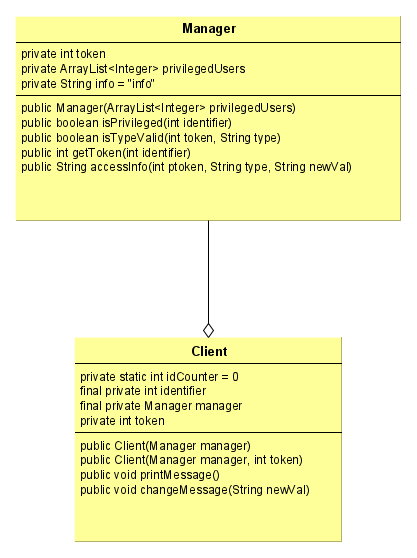
\includegraphics[width=.7 \columnwidth]{utils/Prototype.png}
%    \caption{Functional code for Authenticator pattern}
%    \label{fig:manager_client}
%\end{figure}

%For execution, three clients and a manager are created. The first one is known to the manager as privileged. The second is not privileged. The third one does not authenticate but has the security token (it is for example the case of an attacker who would have succeeded in stealing the security token). Each of these clients then tries to change the value of the resource.

%When the code is executed without JML assertions, the results are final. The third user manages to change the value of the resource. This behavior is perfectly normal since he has the right security token. Indeed, the simple implementation of patterns as described in the UML class diagrams in section 1.3 does not secure the application. In particular, it does not protect the system against identity theft. However, when JML assertions are enabled, the problem is detected as an invariant breach and the program stops.

%Thus, we can see that even in a really simple case, the simple implementation of security patterns is not enough to guarantee the security of the application. However, the verification of the formal contracts defined previously allows to protect against more attacks.

%However, the OpenJML option is not perfect. Indeed, since JML is defined for specification purposes and according to the DbC approach, it is not designed for security. Following limitations are observed:
%\begin{itemize}
 %   \item Some clauses does refer to an assembly of classes, and not a unique class, making impossible to be expressed using JML. A possible workaround is to refactor initial code, but it contradicts our initial requirement to secure existing functional code without being intrusive.
 %   \item For the same reasons, it is really difficult to handle delegation contracts.
 %   \item For some clauses, we need to reference all the instances of a particular concept, and not only the current one (eg P1: uniqueness of Authentication information/Subject pairs).
%    \item Some clauses require a temporal window to be expressed, which is not possible yet.
%\end{itemize}

%For those reasons, we have decided to experiment another approach related to Java annotations, the PAMELA framework \cite{}.

% Sylvain
% Ce serait bien de voir des annotations JML (sur la base d'un code déjà existant)
% Ce serait bien de faire le lien entre ces annotations et les clauses de contrat qu'on a mises en évidence avant, afin de voir ce qu'on peut exprimer, et ce qu'on ne peut pas
% Expliciter ensuite toutes les limitations, et pourquoi on ne peut pas le faire avec JML


% References sur PAMELA

% TODO: est ce qu'on présente PAMELA comme une implem' du MOP (Meta Object Protocol) ?

%PAMELA offers several features, such as:
%\begin{itemize}
%    \item Full life-cycle management of model objects (construction, destruction)
 %   \item Multiple inheritance and traits programming
  %  \item Embedding management and cloning support
   % \item Integrated fine notification support
    %\item Persistence support
    %\item Object graph closure computation, comparison and diff-merge support
    %\item Meta-programming support
    %\item Multi-level UNDO/REDO stack
%\end{itemize}



\section{Experimentation}

In this section, we present an experimentation based on a real use case where cyber-contracts are applied on a legacy code base, based on web Spring framework.

Présenter ici le UC.




\section{Related work}
% Positionnement par rapport aux SecurityPatterns

Développer un peu plus, notamment sur la partie Monitoring@runtime


The security by design approach is mainly based on security patterns applied to many phases of the development process. Several publications focus on security patterns, in general or specific domains such as Yoder and al. \cite{yoder1997}, Fernandez-Buglioni \cite{fernandez2013}, and Yoshioka et al. \cite{yoshioka2008}. In most cases, the patterns are defined based on the original approach of the Gang of Four \cite{gamma1995} with textual definitions and usually represented with refined and stereotyped UML diagrams (Class diagrams for the structural part and Sequence diagrams to represent the behavior of the patterns).

Formal definitions of security patterns are also provided by several authors \cite{cheng2019}, \cite{behrens2018}, \cite{daSilva2013}. In most cases, the purpose of these formal definitions is to analyze the behavior of the patterns at design level or enabling automatic analysis operations. Our proposal to formalize security patterns with a design by contract approach aims at ensuring a secure implementation of patterns. Therefore, this work complements the previous efforts to formalize security patterns.

Originally, the design by contract approach was defined to support reliability on object oriented applications \cite{meyer1992applying}. Then, it was also extended to component modeling \cite{beugnard1999} and formal definitions \cite{mouelhi2019}. 
At code level, the DbC approach is implemented with the JContractor \cite{karaorman2005} framework, which provides run-time contract checking by instrumenting the bytecode of Java classes that define contracts. It however remains limited to the initial scope of Meyer's contracts; i.e., classes and methods. The closest approach to our work is the Aspect Oriented Programming (AOP) approach used by Hallstrom and al. \cite{hallstrom2004} to monitor the pattern contract.
Each pattern contract is associated with a dedicated pattern and is defined in an \emph{aspect}. This \emph{aspect} is used to monitor, at run-time, the applied pattern. Nevertheless, this approach is exclusively focused on the implementation without a will to provide abstraction related to the contract definition. Thus, our formal definition could be used to target such AOP implementations by providing the missing abstraction. 

To the best of our knowledge, the design by contract approach extended to security patterns, associated with a formal definition of the security properties was never used to improve the security of software system, at source code level.

% A finaliser

%Regarding the implementation the most closer approach is based on aspect programming and Jcontractor framework. 
%The MOP approach is also closed relative to the capacity to inspect execution at run-time.





\section{Conclusion}

TODO

%In this paper, we presented a design by contract approach to formalize security patterns. This novel approach improves the behavioral definition of the security patterns and therefore enforces the security of systems at the source code level. 

%The ambition of this article was to address two issues regarding the security of code through the use of security patterns. Our formalization of both functional and implicit parts of security design patterns allowed us to address the first challenge. Our contracts thus provides an explicit description of security patterns which captures tacit elements of the pattern, usually undocumented. The second targeted issue is largely addressed through our PAMELA experiment. We indeed provided an implementation allowing for run-time contract enforcement based on code annotation. Such active monitoring contributes to ensuring pattern security properties in legacy code.

%%One strength of the approach presented in this paper is that it formalizes the definition of both functional behaviors and implicit parts of security design patterns. The latter is even more important since this tacit knowledge is usually not documented in security pattern definitions and therefore not always known by developers.

%%The second issue that we have identified regarding the security of legacy code, is largely addressed through our PAMELA experiment based on code annotation and run-time contract enforcement.

%%A second strength is the ease of implementing the proposal in annotational languages such as JML and PAMELA. 

%% Sylvain: surtout dire qu'on le fait à partir d'une base de code fonctionnel existante, avec des composants logiciels qui n'ont pas été développé en prenant en compte des préoccupation de sécurité, c'est à mon avis ca le principal intérêt de l'approche.

%%Even if the application of the proposal in a proof of concept case highlights the security improvement on  legacy source code, further research is needed to prove the merits of our approach; \textit{e.g.}, its effectiveness and its scalability to real cases. 

%As a future work, we plan to investigate about the use, strengths and weaknesses of our approach with real cases (e.g., Web applications exposed to cyber attacks) to evaluate its scalability and effectiveness.

%%
%% The next two lines define the bibliography style to be used, and
%% the bibliography file.
\bibliographystyle{ACM-Reference-Format}
\bibliography{Contract-SecurityPatterns-MOP}

\end{document}
\endinput
%%
%% End of file `sample-sigchi.tex'.
